\subsection{B2C: Gesteuerter Zweipuls-Gleichrichter}

% --- bestehende Grafik: B2C Schaltung ---
\begin{center}
    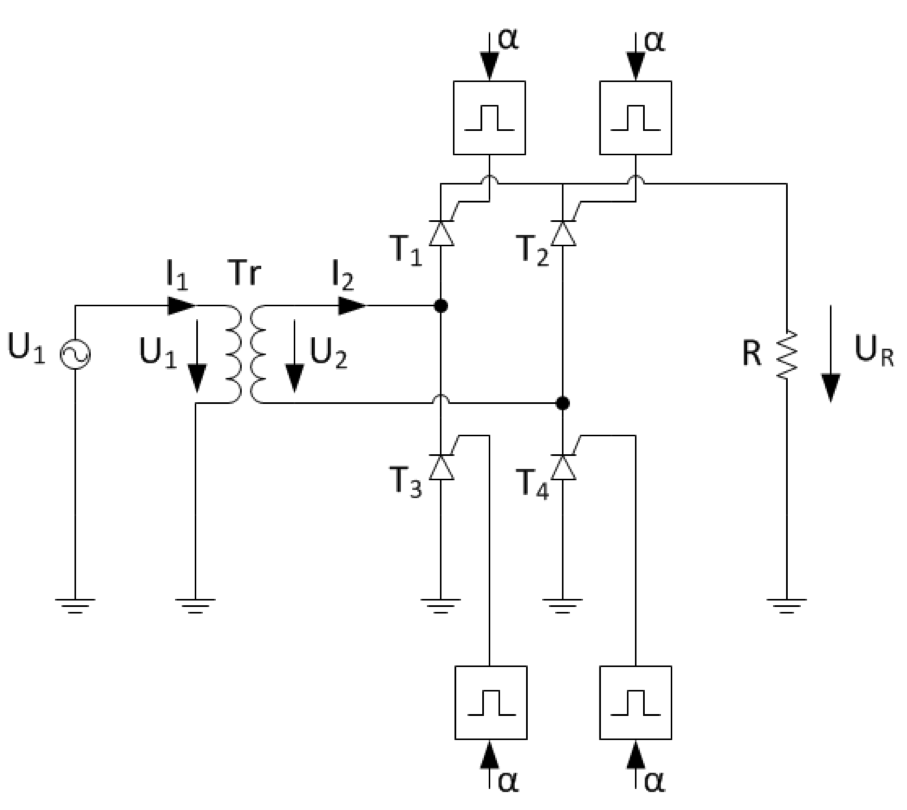
\includegraphics[width=0.85\linewidth]{images/B1C.png}
\end{center}

Der B2C-Gleichrichter verwendet Thyristoren anstelle von Dioden.
Die Gleichspannung ist über den Zündwinkel $\alpha$ steuerbar.

Momentane Ausgangsspannung:
\[
u_d(t) =
\begin{cases}
u_s(t), & \omega t \ge \alpha \\
0, & \omega t < \alpha
\end{cases}
\]

Mittelwert:
\[
\cbl{\overline{u_d} = \frac{2\hat U}{\pi}\cos\alpha}
\]

Eigenschaften:
\begin{itemize}
    \item Stellbereich: $0 \le \alpha \le \pi$
    \item Bei $\alpha > 90^\circ$: Rückspeisebetrieb möglich
    \item Phasenanschnittsteuerung
\end{itemize}

% --- bestehende Grafik: Zündwinkeldiagramm ---
\begin{center}
    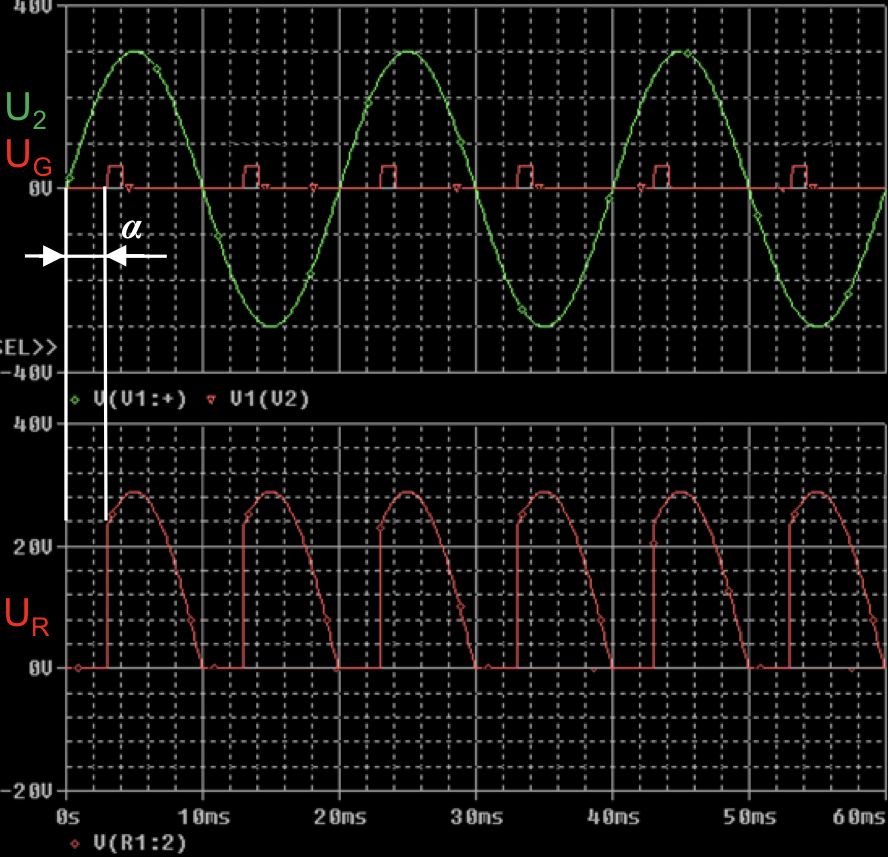
\includegraphics[width=0.85\linewidth]{images/B1C_Verlauf.png}
\end{center}
% -------------------------------------------------

\subsection{Vergleich B2U -- B2C}

\begin{center}
\begin{tabular}{l|c|c}
 & B2U & B2C \\ \hline
Bauelement & Diode & Thyristor \\
Steuerbar & nein & \cbl{ja} \\
Stellgrösse & keine & Zündwinkel $\alpha$ \\
Rückspeisung & nein & möglich \\
\end{tabular}
\end{center}
